\section{Approach}
\label{sec:approach}

We next present our approach for discovering 
likely mappings of API methods  across APIs. 
Figure~\ref{fig:approachOverview} provides an overview of the \tool\ approach.
The \tool\ approach consists of three major components: 1) an Indexer; 2) Query Builder; and 3) Searcher components.


The Indexer accepts the API documents of the target API
and creates indexes (a vector space model) of these documents 
by extracting intermediate contents from the method descriptions. 
The Query Builder accepts the API documents of the source API
and creates queries to be executed on the indexes (a vector space model).
Finally, Searcher component executes the queries on the indexes and 
generates a ranked list of the API methods from target API documents as
mapping results to be presented to the developers for confirmation. 
We next describe each component in detail.


\begin{figure}
	\begin{center}
		%\begin{framed}
		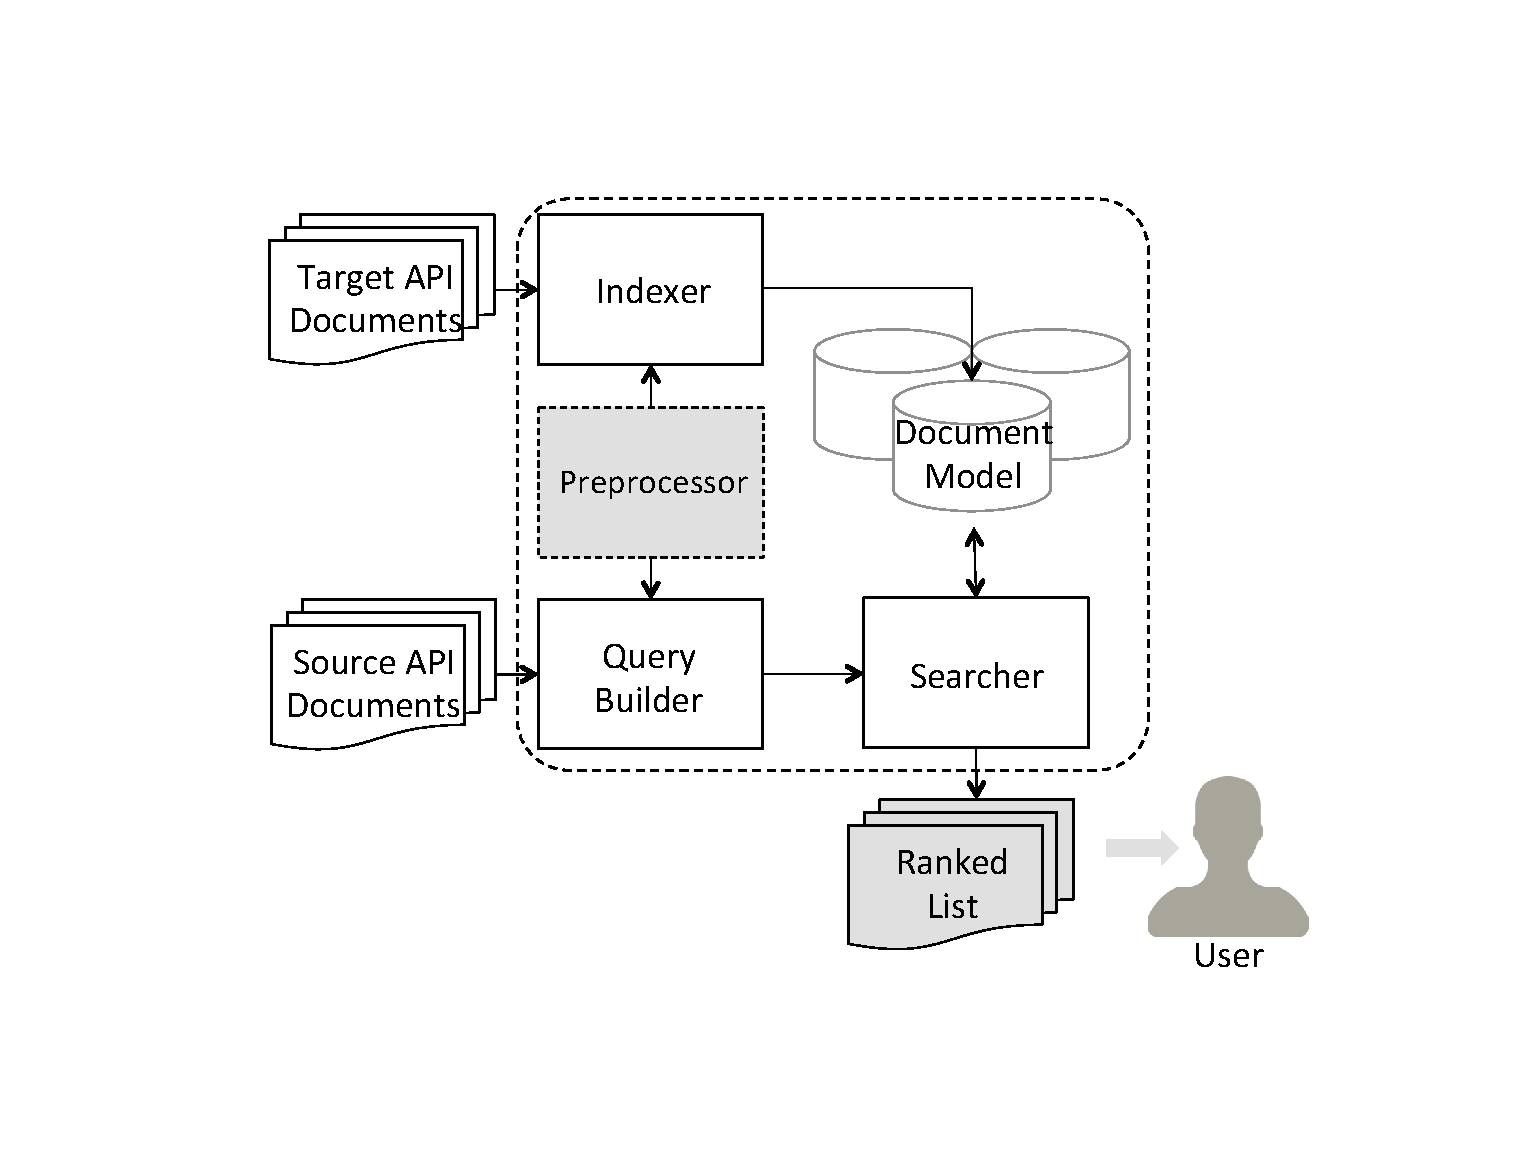
\includegraphics[scale=0.45,clip=true, trim=120pt 80pt 10pt 80pt]{ApproahOverview.eps}
		%\end{framed}
		\vspace*{-4ex}
		\caption{\label{fig:approachOverview} Overview of \tool\ approach}
	\end{center}
	\vspace*{-4ex}
\end{figure}


\subsection{Indexer}
\label{sub:Approach_Indexer}

This component accepts the API method descriptions of the target API
and creates indexes (a vector space model) of these documents.
In particular, Indexer extracts the following fields from the API method descriptions:

 
\textbf{F1) Type Name}: The name of enclosing class/interface of the method. For the method description of \CodeIn{drawString} shown in Figure~\ref{fig:drawStringJavadoc}, indexer extracts the type Name as ``Graphics''.
	
\textbf{F2) Package Name}: The package name of the enclosing type. For the method description shown in Figure~\ref{fig:drawStringJavadoc}, indexer extracts the package name as ``javax.microedition.lcdui''.
	
\textbf{F3) Method Name}: The name of the method. For the method description shown in Figure~\ref{fig:drawStringJavadoc}, indexer extracts the method name as ``drawString''.
	
%	\item \textbf{F4) Method Modifiers}: The access modifiers of the method. For the method description shown in Figure~\ref{fig:drawStringJavadoc}, indexer extracts the method modifiers as ``public''.
%	
%	\item \textbf{F5) Method Return Type}: The return type of the method. For the method description shown in Figure~\ref{fig:drawStringJavadoc}, indexer extracts the return type as ``void''.
%	
%	\item \textbf{F6) Exceptions Thrown}: Name of the exceptions thrown by the method. For the method description shown in Figure~\ref{fig:drawStringJavadoc}, indexer extracts the exception names as ``NullPointerException'' and ``IllegalArgumentException''.
%	
%	\item \textbf{F7) Parameters}: The name and type information of parameters. For the method description shown in Figure~\ref{fig:drawStringJavadoc}, indexer extracts the parameter name and type information as ``String str'',``int x'',``int y'', and ``int anchor''.
	
\textbf{F4) Class Description}: The description of enclosing type. Class description is not shown in Figure~\ref{fig:drawStringJavadoc} for the space considerations.
	
\textbf{F5) Method Description}: The description of the method. For the method description shown in Figure~\ref{fig:drawStringJavadoc}, indexer extracts the method description as the all the text except method declaration in Line 1.


This step is required to extract the desired descriptive text from the API method descriptions.
Getting structured descriptions facilitates searching on individual categories.
This step allows \tool\ to deal with the \textit{structure} issue as presented in Section~\ref{sec:example}.
Different API documents may have different styles of presenting information to developers.
Such stylistic differences may also include the difference in the level of the details presented to developers.
\tool\ relies only on basic fields that are generally available for API methods across different presentation styles. 

After extracting the desired information, extracted text is further preprocessed.
The preprocessing steps are required to make the text amenable to text mining techniques
that are used in the subsequent phases of the \tool\ approach.
In particular, \tool\ performs the following basic prepossessing steps: 

\textbf{P1) Presentation Elements}: A typical API method description is often interleaved with presentation elements for better readability. For instance, \CodeIn{JavaDoc} provides a list of identifiers such as  \CodeIn{@Code} and  \CodeIn{@link}. These identifiers are automatically translated into presentation markup, such as links and fonts. Although such elements are part of the description text, these elements often cause noise in the text mining techniques to compute relevance based on the query. Therefore, this preprocessing step cleans the method descriptions to remove such elements. We use a static list of presentation elements to achieve cleaning in this step with relatively high accuracy.
	
\textbf{P2) Split Package Notation}: In method descriptions, the ``.'' character is used as a separator character for package names like ``\CodeIn{javax.microedition.lcdui}''. We use regular expressions to split the package name into constituent words to facilitate search on individual words in the package name. For example, ``\CodeIn{javax.microedition.lcdui}'' is split into ``javax microedition lcdui''.

\textbf{P3) Split CamelCase Notation}: API method descriptions are often interleaved with programming identifiers, such as class names and method names.
Oftentimes these identifiers use CamelCase notation.
The CamelCase notation is the \textit{de facto} mechanism used by programmers for combining phrases into a single word, such that each word in the phrase begins with a capital letter.
Previous research~\cite{Little2009} demonstrated the benefit of splitting the CamelCase word into its constituent phrase for automated code completion.
\tool\ splits such identifiers into constituent phrases to better facilitate searching.
\tool\ leverages the well-formed structure of CamelCase notations to encode a regular expression to achieve splitting with relatively high accuracy.
For example, ``\CodeIn{drawString}'' is split into ``draw String''.   

\textbf{P4) Lowercase}: This step involves converting the text description to lower case. The step is performed to normalize the text for making the keyword match case insensitive, further increasing the range of queries.
	
\textbf{P5) Stemming}: This steps transforms the words in the description to their base form. Stemming is very effective in extending the range of keyword based queries to match various operational forms of the words. For instance, ``has'', ``have'', and ``had'' are mapped to the stem ``ha''. We use the default implementation of the Lucene Porter stemmer for indexer. 
	


After preprocessing, \tool\ next creates indexes for the API method descriptions.
An index is collection of documents where each document is made up of 
values organized into well defined fields.
\tool\ considers every method description as an individual document and 
uses the following major fields (as previously described):
1) combination of package and class name;
2) class description;
3) method signature;
4) method name; and
5) method description.
The values are of these fields is text after preprocessing.
\tool\ uses a vector space model representation of the documents for each field. 
Vector space model or term vector model is an algebraic model for representing text documents (and any objects, in general) as vectors of identifiers and their frequency of occurrence. 
In case of \tool, each word is considered as a term except the stop words, such as ``a'', ``the'', and ``and''.


  

\subsection{Query Builder}
\label{sub:Approach_Searcher}

This component accepts the API method descriptions of the source API
and creates queries for method descriptions.
These queries are executed on the target API index to retrieve 
an ordered list relevant API methods.
In particular, Query Builder uses the same preprocessing steps followed by Indexer
(listed in Section~\ref{sub:Approach_Indexer}).
After extracting the desired descriptive text from the API method descriptions,
this component systematically creates search queries to search for different fields in Indexes.
Keywords for searching in ``Type Name'', ``Type Description'', ``Method Name'', and ``Method Description'' fields are derived from their equivalents in the extracted descriptive text.


For instance, consider the method description shown in  Figure~\ref{fig:hasNextJavadoc} 
and equivalent query in shown in Figure~\ref{fig:hasNextJavaQuery}.
The Keywords for ``Type Name'' are derived from preprocessing ``java.util.Iterator'' resulting in ``\CodeIn{java util iter}''. Notice the package notation is split into individual words and ``Iterator'' is further transformed to lower case and its stem ``iter''.
Likewise, keywords for field ``Method Name'' is derived by preprocessing ``hasNext'', which is first split into ``has Next'' and then transformed using stemming into ``\CodeIn{ha next}'' (\textit{ha} being stem of word \textit{has}).

\begin{figure}
	\begin{framed}
		{\small java.util} Interface Iterator {\LARGE hasNext}\\
		\CodeIn{boolean hasNext()}\\
		Returns \CodeIn{true} if the iteration has more elements. (In other words, returns true if \CodeIn{next()} would return an element rather than throwing an exception.)\\
		\textbf{Returns}:\\
		\CodeIn{true} if the iteration has more elements
	\end{framed}
	\vspace{-2ex}
	\caption{API Method Description of \CodeIn{hasNext} method in \CodeIn{Iterator Interface} from Java API}
	\label{fig:hasNextJavadoc}
	\vspace{-2ex}
\end{figure}

\begin{figure}
	\begin{framed}	
		\textbf{Type Name}: \CodeIn{java util iter}\\
		\textbf{Type Description}: \CodeIn{iter over collect iter take enumer java collect framework}\\
		\textbf{Method Name}: \CodeIn{ha next}\\
		\textbf{Method Description}: \CodeIn{return true iter ha more element other word return true next would return element rather than throw except}
	\end{framed}
	\vspace{-2ex}
	\caption{Query based on API method description of \CodeIn{hasNext} method in \CodeIn{Iterator Interface} from Java API}
	\label{fig:hasNextJavaQuery}
	\vspace{-4ex}
\end{figure}


For generating keywords to query the ``Type Description'' field we consider following heuristic:
\textit{Heuristic H1:  the first paragraph or the first five sentences of the type description (whichever is shorter) provides reasonable keywords for searching equivalent class in target API.} 

Likewise, for generating the keywords to query the ``Method Description'' field, we consider the following heuristic: \textit{Heuristic H2: the first paragraph or the first two sentences of the method description (whichever is shorter) provides reasonable keywords for searching equivalent method in target API.}

\tool\ uses these heuristics to improve the performance of searching infrastructure
that tends to be inversely proportional to the complexity and length of the query.
Using all the descriptive text as keywords results in a verbose query.
As the number of keywords in a query increases the effectiveness of the query decreases.
A large number of keywords have higher probability of matching large number of documents in comparison to a query with fewer keywords.
In contrast, we observed that the document writers tend to describe the general
overview of class and method description in the first few sentences followed by implementation and design specific details.
We thus focused on the words in these overview sentences to create queries instead of using entire descriptive text.


\textbf{Weights for terms}. As mentioned in Section~\ref{sec:example},
all terms in a method description are not equally important keywords. 
\tool\ further enhances the query by quantifying the importance of a term in the method description and use that as the weight of the corresponding keywords in the query.
In particular, we propose to use tf-idf\cite{manning2008introduction} as a means to quantify importance of a term.
For each term in the method description \tool\ calculates the number of times the term occurs in that method description as $freq_{mtd}$.
\tool\ also calculates the maximum frequency of any term in the document as $freq_{MAX}$.
\tool\ then calculates the number of documents in the corpus that contains the term as $freq_{doc}$.
\tool\ finally calculates the tf-idf score of the term (as listed \cite{manning2008introduction}) as:

\begin{center}
	\CodeIn{tf-idf} = $(0.5\ +\dfrac{0.5\ X\ freq_{mtd}}{freq_{MAX}})\ * log(1\ +\ \dfrac{total_{mtd}}{freq_{doc}})$
\end{center}

The calculated tf-idf values of terms are normalized to a range of 0 to 1 (both 0 and 1 inclusive) for each document.
The normalized tf-idf sore of the top-k term is then used as the weights for the corresponding  keywords occurring in the query.

For the API method description  shown in Figure~\ref{fig:hasNextJavadoc}, \tool\ calculates ``iter'', ``ha'' (Lemma of ``has''), and ``element'' as most the important terms with normalized tf-idf scores of 1.0, 1.0, and 0,6 respectively. We augment the query shown in Figure~\ref{fig:hasNextJavaQuery} with the computed weights for the keywords respectively.

\subsection{Searcher}
\label{sub:approach_searcher}

The searcher component accepts the query from Query Builder component and queries the index generated by Indexer component.
The results are then ranked and presented to the end user for review.
The searcher is realized as follows. 
First all the documents that match the keywords and clauses in a query are returned.
Then, the returned documents are ranked using the cosine similarity\cite{singhal2001modern} of the terms in query and the terms in returned documents. In mathematics, Cosine similarity is a numerical statistic to measure the similarity between two vectors. 
In information theory~\cite{manning2008introduction}, cosine similarity is the standard statistic to rank relevant documents.




    


\subsection{Implementation}
\label{sub:Approach_implementation}

We implemented a prototype version of the \tool\ approach.
We first manually download the HTML version of API documents of libraries. 
We then implemented a parser for extracting the requisite text from these documents using 
Jsoup~\footnote{\url{http://jsoup.org/}}, which is a java library for working with HTML documents.
In particular our prototype implementation parses: 
1) Oracle's Javadoc style;
2) Android style documentation; and
3) Microsoft's  MSDN documentation.

We next implemented the indexing, query building, and searching infrastructure using the Apache Lucene~\cite{lucene}.
Lucene is a high-performance, full-featured text search engine library written entirely in Java.
Our prototype implementation and evaluation subjects are publicly available on the project website~\footnote{\url{https://sites.google.com/a/ncsu.edu/apisim/}}. 
